\documentclass{plt}
\usetheme{metropolis}           % Use metropolis theme

\tikzset{double distance=1pt,>=latex}

\tikzset{
  parsetree/.style={
    level distance=2pc,
    sibling distance=1.8pc,
    every node/.style={fill=white},
    every path/.style={thick},
    baseline=(current bounding box.west)
  }
}

% Make | a mathrel symbol: improves alternation (a | b) spacing
\mathcode`\|="326A

\def\filled#1{\ifx#11mRed\else white\fi}

%\DeclareSymbolFont{operator}{OT1}{put}{m}{n}
%\DeclareSymbolFont{letters}{OT1}{put}{m}{it}

% For drawing arithmetic parse trees

\def\plus#1#2{node {\texttt{+}} child {#1} child {#2}}
\def\minus#1#2{node {\texttt{-}} child {#1} child {#2}}
\def\mult#1#2{node {\texttt{*}} child {#1} child {#2}}
\def\lit#1{node {#1}}

\tikzfading[name=fade down,
  top color=transparent!0,
  bottom color=transparent!100]

\tikzfading[name=fade up,
  bottom color=transparent!0,
  top color=transparent!100]

\newcommand{\pac}{\begin{tikzpicture}
    \draw [fill=black!30!mBlue!100] (2.12pt,2.12pt) arc
    (45:315:3pt) -- (0,0) -- cycle;
  \end{tikzpicture}
}

\if 0
\newcommand{\handle}[3]{
  \begin{tikzpicture}
    \node [inner sep=1pt] (n1) {$#1$};
    \node [inner sep=1pt,anchor=base west] (n2) at (n1.base east) {$#2$};
    \node [inner sep=1pt,anchor=base west] (n1) at (n2.base east) {$#3$};
    \begin{pgfonlayer}{background}
      \draw [mRed!70,line width=2pt,rounded corners]
      ($(n2.north east) + (1pt,1pt)$) --
      ($(n2.north west) + (-1pt,1pt)$) --
      ($(n2.south west) + (-1pt,-1pt)$) --
      ($(n2.south east) + (1pt,-1pt)$) -- cycle
      ;
    \end{pgfonlayer}
  \end{tikzpicture}
}
\fi

\newcommand{\expand}[3]{
    \fill [even odd rule,mRed,path fading=fade up]
    (#1.north west)  [rounded corners] -- (#1.south west) --
    (#2.north west) -- (#2.south west) -- (#3.south east) --
    (#3.north east) -- (#1.south east) -- (#1.north east)
    -- cycle
    ($(#3.north east) + (-1pt,-1pt)$) --
    ($(#2.north west) + (1pt,-1pt)$) --
    ($(#2.south west) + (1pt,1pt)$) --
    ($(#3.south east) + (-1pt,1pt)$) -- cycle
    ;
}

\newcommand{\expandup}[3]{
    \fill [even odd rule,mRed,path fading=fade down]
    (#1.south west)  [rounded corners] -- (#1.north west) --
    (#2.south west) -- (#2.north west) -- (#3.north east) --
    (#3.south east) -- (#1.north east) -- (#1.south east)
    -- cycle
    ($(#3.south east) + (-1pt,1pt)$) --
    ($(#2.south west) + (1pt,1pt)$) --
    ($(#2.north west) + (1pt,-1pt)$) --
    ($(#3.north east) + (-1pt,-1pt)$) -- cycle
    ;
}



\newcommand{\id}{\textbf{Id}}

\newcommand{\grammarone}{
\renewcommand{\arraystretch}{1}
$\begin{array}[t]{@{}l@{\,}r@{\,}c@{\,}l@{}}
1: & e & \rightarrow & t + e \\
2: & e & \rightarrow & t \\
3: & t & \rightarrow & \id\ * t \\
4: & t & \rightarrow & \id
\end{array}$
}


\newenvironment{parsermoves}{
\begingroup
\small
\renewcommand{\arraystretch}{0.8}
\newcommand{\s}[2]{%
  \begin{pspicture}(10pt,10pt)
    \psframe(0,-5pt)(8pt,5pt)
    \rput(4pt,2pt){\tiny##1}
    \rput(4pt,-2pt){\tiny##2}
  \end{pspicture}}
\begin{tabular}[t]{l@{}rl}
\multicolumn{1}{c}{\hbox to 5em{\hss stack\hss}} & \multicolumn{1}{c}{input}
& \multicolumn{1}{c}{action} \\
}{
\end{tabular}
\endgroup
}


\title{Scanner}
\author{Ronghui Gu}
\institute{Columbia University}
\date{Spring 2019}
\titlegraphic{
\vspace{220pt}
{\tiny $^*$ Course website: \url{https://www.cs.columbia.edu/~rgu/courses/4115/spring2019}\vspace{-5pt}}\\
{\tiny $^{**}$ These slides are borrowed from Prof. Edwards.}
}

\begin{document}

\frame{\titlepage}


\tikzset{
    mymodule/.style={draw, fill=white, drop shadow},
    code/.style={draw, fill=gray!15, drop shadow,minimum width=0},
    emph/.style={draw, fill=mBlue!15, drop shadow},
}

\part{The Big Picture}

\begin{frame}{The First Question}
  \begin{center}
    \large How do we describe/construct a program?
%    \vspace{5pc}
%
%    \emph{Compilers should accept many programs; \\
%      how do we describe which one we want?}
  \end{center}
\end{frame}

\begin{frame}{Use continuously varying values?}
  \begin{center}
    \includegraphics[width=0.5\textwidth]{edison-phonograph.jpg}

    Very efficient, but has serious noise issues

    \tiny Edison Model B Home Cylinder phonograph, 1906
    
  \end{center}
\end{frame}

\begin{frame}{The ENIAC: Programming with Spaghetti}

  \includegraphics[width=\textwidth]{eniac4.jpg}

\end{frame}

\begin{frame}{Have one symbol per program?}
  \begin{center}
    \includegraphics[width=0.75\textwidth]{Sholes-Glidden.jpg}

    Works nicely when there are only a few things

    \tiny Sholes and Glidden Typewriter, E. Remington and Sons, 1874

  \end{center}
\end{frame}

\begin{frame}{Have one symbol per program?}
  \begin{center}
    \includegraphics[width=0.6\textwidth]{Japanese_typewriter_SH-280.jpg}
    \hfill
    \includegraphics[scale=0.5,viewport=900 400 1100 745,clip]%
                    {Japanese_typewriter_SH-280.jpg}

    Not so good when there are many, many things

    \tiny Nippon Typewriter SH-280, 2268 keys

  \end{center}
\end{frame}

\begin{frame}{Solution: Use a Discrete Combinatorial System}

Use \alert{combinations} of a \alert{small number of things} to
represent (exponentially) many different things.

\begin{minipage}{0.2\textwidth}
\includegraphics[width=\textwidth]{dna-overview-clean.png}
\end{minipage}%
\begin{minipage}{0.8\textwidth}
\hfill
\includegraphics[width=0.3\textwidth]{rosetta-stone.jpg} \hfill
\includegraphics[width=0.5\textwidth]{English-sounds.png}

\hfill
\includegraphics[width=0.4\textwidth]{cells.jpg}
\hfill
\includegraphics[width=0.4\textwidth]{silicon-atoms.jpg}
\end{minipage}

\end{frame}

\begin{frame}[fragile]{Every Human Writing System Does This}

\tiny

\begin{tabular}{ccc}
\includegraphics[width=0.3\textwidth]{hieroglyphics-at-karnak-tem.jpg} &
\includegraphics[width=0.3\textwidth]{FMW-Cuneiform-Tablet-3.jpg} \\
Hieroglyphics (24+) & Cuneiform (1000 -- 300) \\ \\
\includegraphics[width=0.3\textwidth]{sanskrit-inscription-prasat-kravan.jpg}
&
\includegraphics[width=0.3\textwidth]{chinese-stela-inscription.jpg}
&
\includegraphics[width=0.25\textwidth]{IBM-Selectric-Element.jpg}
\\
Sanskrit (36) & Chinese (214 -- 4000) & IBM Selectric (88--96) \\ \\
\includegraphics[width=0.3\textwidth]{mayan-palenque-glyphs-edit1.jpg} &
\includegraphics[width=0.3\textwidth]{Trajan_inscription.jpg} \\
Mayan (100) & Roman (21--26) \\
\end{tabular}

\end{frame}

\begin{frame}{The Second Question}
  \begin{center}
  How do we describe the \alert{combinations} of a \alert{small number of things}.

  \end{center}
\end{frame}

\begin{frame}{Just List Them?}

  \includegraphics[width=\textwidth]{Oxford-English-Dictionary.jpg}

  Gets annoying for large numbers of combinations

\end{frame}

\begin{frame}{Just List Them?}
  \begin{center}    
    \includegraphics[width=0.85\textwidth]{aaaaaaa.png}
  
    Can be really redundant
  \end{center}
\end{frame}

\begin{frame}[fragile,t]{Scanning and Parsing}

\begin{center}
\hspace{20pt}
\begin{tikzpicture}
  \matrix [matrix of nodes,
           row sep=0.8pc,
           column sep=2pc,
           every node/.style={draw, fill=white, drop shadow,minimum width=5.5cm}] {
     |[code] (b)| int avg (int a, int b) ... \\
     |[emph] (a)| Lexical Analysis \\
     |[emph] (aa)| Syntax  Analysis \\
     |(aaa)| Semantic Analysis \\
     |(a4)| Intermediate Code Generation \\
     |(a5)| Optimization \\
     |(a6)| Code Generation \\
    |[code] (c)| 0101110101... \\
  };
  \begin{scope}[->]
    \draw (b) -- (a);
    \draw (a) -- (aa);
    \draw (aa) -- (aaa);
    \draw (aaa) -- (a4);
    \draw (a4) -- (a5);
    \draw (a5) -- (a6);
    \draw (a6) -- (c);
  \end{scope};
  \begin{scope}[densely dotted]
    \draw (-10pc,-2.6pc) -- (10pc,-2.6pc);
    \draw (-10pc,-5pc) -- (10pc,-5pc);
  \end{scope};
  \node at (9pc,0) {front-end};
  \node at (9.5pc,-4pc) {middle-end};
  \node at (9pc,-6pc) {back-end};
\end{tikzpicture}
\end{center}

\end{frame}


\part{Lexical Analysis}

\begin{frame}[fragile]{Lexical Analysis (Scanning)}

Translate a stream of characters to a stream of tokens

\includegraphics[width=0.5\textwidth]{subway-tokens.jpg}

\def\sp{{\tt\char`\ }}

\begin{semiverbatim}
f o o \sp = \sp a + \sp bar ( 0 , \sp 42 , \sp q ) ;
\end{semiverbatim}

\newcommand{\token}[1]{\tikz \node [minimum height=15pt,draw,rounded corners=2pt,fill=mBlue!10] {#1};}

\token{ID}
\token{EQUALS}
\token{ID}
\token{PLUS}
\token{ID}
\token{LPAREN}
\token{NUM}
\token{COMMA}
\token{ID}
\token{LPAREN}
\token{SEMI}

\medskip

\begin{tabular}{lll}
\toprule
\textbf{Token} & \textbf{Lexemes} & \textbf{Pattern} \\
\midrule
EQUALS & \texttt{=} & an equals sign \\
PLUS & \texttt{+} & a plus sign \\
ID & \texttt{a foo bar} & letter followed by letters or digits \\
NUM & \texttt{0 42} & one or more digits \\
\bottomrule
\end{tabular}

\end{frame}

\begin{frame}[fragile,t]{Lexical Analysis}

Goal: simplify the job of the parser and reject some wrong programs, e.g.,

\begin{C}
%#@$^#!@#%#$
\end{C}

is not a C program$^\dagger$

Scanners are usually much faster than parsers.

Discard as many irrelevant details as possible (e.g., whitespace, comments).

Parser does not care that the  identifer is
``supercalifragilisticexpialidocious.''

Parser rules are only concerned with tokens.

\vfill

\footnotesize
$^\dagger$ It is what you type when your head hits the keyboard

\end{frame}

\begin{frame}{Describing Tokens}

\textbf{Alphabet}: A finite set of symbols

Examples: $\{$ 0, 1 $\}$, $\{$ A, B, C, \ldots, Z $\}$, ASCII, Unicode

\vspace{2pc}

\textbf{String}: A finite sequence of symbols from an alphabet

Examples: $\epsilon$ (the empty string), Ronghui, $\alpha\beta\gamma$

\vspace{2pc}

\textbf{Language}: A set of strings over an alphabet

Examples: $\emptyset$ (the empty language), $\{$ 1, 11, 111, 1111
$\}$, all English words, strings that start with a letter followed by
any sequence of letters and digits

\end{frame}

\begin{frame}{Operations on Languages}

Let $L = \{$ $\epsilon$, wo $\}$, $M = \{$ man, men $\}$

\vspace{1pc}

\textbf{Concatenation}: Strings from one followed by the other

$LM = \{$ man, men, woman, women $\}$

\vspace{1pc}

\textbf{Union}: All strings from each language

$L \cup M = \{ \epsilon, $ wo, man, men $\}$

\vspace{1pc}

\textbf{Kleene Closure}: Zero or more concatenations

$M^* = \{ \epsilon \} \cup M \cup MM \cup MMM \cdots = \break
 \{ \epsilon, $ man, men, manman, manmen, menman, menmen,
manmanman, manmanmen, manmenman, \ldots $\}$

\end{frame}
%
%\begin{frame}{Kleene Closure}
%
%\begin{columns}
%\begin{column}{0.65\textwidth}
%\raggedright
%
%``*'' is named after Stephen Cole Kleene, the inventor of regular
%expressions, who pronounced his last name ``CLAY-nee.''
%
%\medskip
%
%His son Ken writes ``As far as I am aware this pronunciation is incorrect
%in all known languages. I believe that this novel pronunciation was
%invented by my father.''
%\end{column}
%\begin{column}{0.45\textwidth}
%\includegraphics[width=\textwidth]{kleene.jpg}
%\end{column}
%\end{columns}
%
%\end{frame}

\begin{frame}{Regular Expressions over an Alphabet $\Sigma$}

A standard way to express languages for tokens.

\begin{enumerate}

\item $\epsilon$ is a regular expression that denotes $\{\epsilon\}$

\item If $a \in \Sigma$, $a$ is an RE that denotes $\{a\}$

\item If $r$ and $s$ denote languages $L(r)$ and $L(s)$,

\[
\begin{array}{lll}
(r)|(s) &\textsf{denotes}& L(r) \cup L(s) \\[10pt]
(r)(s) && \{ tu : t \in L(r), u \in L(s) \} \\[10pt]
(r)^* && \cup_{i=0}^{\infty} L(r)^i \\
& \textsf{where} & L(r)^0 = \{\epsilon\}\ \\
& \textsf{and} & L(r)^i = L(r) L(r)^{i-1} \\
\end{array}
\]

\end{enumerate}

\end{frame}

\begin{frame}{Regular Expression Examples}

$\Sigma = \{ a, b \}$

\begin{tabular}{ll}
\toprule
\textbf{Regexp.} & \textbf{Language} \\
\midrule
$a | b$ & $\{ a, b \}$ \\
$(a|b)(a|b)$ & $\{ aa, ab, ba, bb \}$ \\
$a^*$ & $\{ \epsilon, a, aa, aaa, aaaa, \ldots \}$ \\
$(a|b)^*$ & $\{ \epsilon, a, b, aa, ab, ba, bb, aaa, aab, aba, abb,
\ldots \}$ \\
$a | a^*b$ & $\{ a, b, ab, aab, aaab, aaaab, \ldots \}$ \\
\bottomrule
\end{tabular}

\end{frame}

\begin{frame}{Specifying Tokens with REs}

ID: letter followed by letters or digits

\vspace{1pc}

Typical choice: $\Sigma = $ ASCII characters, i.e., $\{
\texttt{\char`\ }, !, \texttt{"}, \#, \$, \ldots, \textrm{0},
\textrm{1}, \ldots, \textrm{9},
\ldots, \textrm{A}, \ldots, \textrm{Z}, \ldots, \texttt{\char`\~} \}$

\textbf{letters}: $\textrm{A} | \textrm{B} | \cdots | \textrm{Z} |
\textrm{a} | \cdots | \textrm{z}$

\textbf{digits}: $\textrm{0} | \textrm{1} | \cdots | \textrm{9}$

\textbf{identifier}: $\textbf{letter}\, (\, \textbf{letter}\, | \,
\textbf{digit}\, )^*$

\end{frame}

\begin{frame}{Implementing Scanners Automatically}

\begin{center}
\begin{tikzpicture}
  \matrix (re) [matrix of nodes,
    row sep=2pc,
    nodes={fill=white,draw,drop shadow}] {
    Regular Expressions (Rules) \\
    Nondeterministic Finite Automata \\
    Deterministic Finite Automata \\
    Tables \\
  };
\draw [->] (re-1-1) -- (re-2-1);
\draw [->] (re-2-1) -- node [right] {Subset Construction} (re-3-1);
\draw [->] (re-3-1) -- (re-4-1);
\end{tikzpicture}
\end{center}

\end{frame}

\begin{frame}[fragile]{Nondeterministic Finite Automata}

\begin{columns}
\begin{column}{0.4\textwidth}

``All strings containing an even number of 0's and 1's''

\vspace{2pc}

\begin{tikzpicture}
  \matrix [matrix of math nodes,
    nodes={circle,draw},
    column sep=2.5pc,
    row sep=2.5pc] {
    |[double] (A)| A & |(B)| B \\
    |(C)| C & |(D)| D \\
  };
  \begin{scope}[->, bend angle=15,bend left,inner sep=2pt]
    \draw (A) to node [above] {0} (B); 
    \draw (B) to node [below] {0} (A);
    \draw (B) to node [right] {1} (D); 
    \draw (D) to node [left]  {1} (B);
    \draw (D) to node [below] {0} (C); 
    \draw (C) to node [above] {0} (D);
    \draw (C) to node [left] {1} (A); 
    \draw (A) to node [right] {1} (C);
    \draw (A) ++ (-1.3pc,1pc) -- (A);
  \end{scope}
\end{tikzpicture}

\end{column}
\begin{column}{0.6\textwidth}

\begin{enumerate}\itemsep=0pt

\item Set of states $S:
\left\{
\begin{tikzpicture}[baseline=-4pt]
  \matrix [column sep=5pt,matrix of math nodes,nodes={circle,draw}] {
    |[double]| A & B & C & D \\ };
\end{tikzpicture}
\right\}$

\item Set of input symbols $\Sigma: \{ 0, 1 \}$

\item Transition function $\sigma : S \times \Sigma_{\epsilon} \rightarrow 2^S$

$\begin{array}{c|ccc}
\textbf{state} & \epsilon & 0 & 1 \\
\hline
A & \emptyset & \{B\} & \{C\} \\
B & \emptyset & \{A\} & \{D\} \\
C & \emptyset & \{D\} & \{A\} \\
D & \emptyset & \{C\} & \{B\} \\
\end{array}
$

\item Start state $s_0 :

\begin{tikzpicture}[baseline=-4pt]
  \node [draw,circle,double] {$A$};
\end{tikzpicture}
 $

\item Set of accepting states $F:
\left\{

\begin{tikzpicture}[baseline=-4pt]
  \node [draw,circle,double] {$A$};
\end{tikzpicture}
\right\}$

\end{enumerate}

\end{column}
\end{columns}

\end{frame}

\begin{frame}[fragile]{The Language induced by an NFA}

An NFA accepts an input string $x$ iff there is a path from the start
state to an accepting state that ``spells out'' $x$.

\vspace{2pc}

\begin{center}
\begin{tikzpicture}
  \matrix [matrix of math nodes,
    nodes={circle,draw},
    column sep=2.5pc,
    row sep=2.5pc] {
    |[double] (A)| A & |(B)| B \\
    |(C)| C & |(D)| D \\
  };
  \begin{scope}[->, bend angle=15,bend left,inner sep=2pt]
    \draw (A) to node [above] {0} (B); 
    \draw (B) to node [below] {0} (A);
    \draw (B) to node [right] {1} (D); 
    \draw (D) to node [left]  {1} (B);
    \draw (D) to node [below] {0} (C); 
    \draw (C) to node [above] {0} (D);
    \draw (C) to node [left] {1} (A); 
    \draw (A) to node [right] {1} (C);
    \draw (A) ++ (-1.3pc,1pc) -- (A);
  \end{scope}
\end{tikzpicture}
\end{center}

Show that the string ``010010'' is accepted.

\begin{tikzpicture}
  \matrix (z) [matrix of math nodes,
    nodes={circle,draw},
    column sep=1.5pc] {
    |[double]| A & B & D & C & D & B & |[double]| A \\
  };
  \begin{scope}[->,every node/.style={above}]
    \draw (z-1-1) -- node {0} (z-1-2);
    \draw (z-1-2) -- node {1} (z-1-3);
    \draw (z-1-3) -- node {0} (z-1-4);
    \draw (z-1-4) -- node {0} (z-1-5);
    \draw (z-1-5) -- node {1} (z-1-6);
    \draw (z-1-6) -- node {0} (z-1-7);
  \end{scope}
\end{tikzpicture}

\end{frame}

\begin{frame}[fragile]{Translating REs into NFAs (Thompson's algorithm)}

% http://hackingoff.com/compilers/regular-expression-to-nfa-dfa

\tikzset{every matrix/.style={matrix of math nodes,
                              nodes={circle,minimum size=1pc,draw}},
         initial text={},
         every state/.style={minimum size=1.5pc,fill=white},
         group/.style={ellipse,draw,fill=mBlue!30,minimum height=2.7pc, inner sep=-5pt},
         node distance=0.5pc and 2pc}

\begin{tabular}{ccc}
$a$ &
\begin{tikzpicture}[baseline=-4pt]
  \node[state,initial]              (A) {};
  \node[state,accepting,right=of A] (B) {};
  \path [->] (A) edge node [above] {$a$} (B);
\end{tikzpicture}
&
Symbol
\\[1pc]
$r_1 r_2$ &
\begin{tikzpicture}[baseline=-4pt]
  \node [state,initial]              (A) {};
  \node [state,right=of A]           (B) {};
  \node [state,accepting,right=of B] (C) {};
  \begin{pgfonlayer}{background}
    \node [group,fit=(A) (B)] {$r_1$};
    \node [group,fit=(B) (C)] {$r_2$};
  \end{pgfonlayer}
  \node [group,fill=none,fit=(A) (B)] {$r_1$};
\end{tikzpicture}
&
Sequence
\\[2pc]
$r_1 | r_2$ &
\begin{tikzpicture}[baseline=-4pt]
  \node [state,initial]              (A) {};
  \node [state,above right=of A]     (B) {};
  \node [state,right=of B]           (C) {};
  \node [state,accepting,below right=of C] (D) {};
  \node [state,below right=of A]     (E) {};
  \node [state,right=of E]     (F) {};
  \begin{pgfonlayer}{background}
    \node [group,fit=(B) (C)] {$r_1$};
    \node [group,fit=(E) (F)] {$r_2$};
  \end{pgfonlayer}
  \path [->] (A) edge node [above left] {$\epsilon$} (B)
             (A) edge node [below left] {$\epsilon$} (E)
             (C) edge node [above right] {$\epsilon$} (D)
             (F) edge node [below right] {$\epsilon$} (D);
\end{tikzpicture}
&
Choice
\\[3pc]
$(r)^*$ &
\begin{tikzpicture}[baseline=-4pt]
  \node [state,initial]              (A) {};
  \node [state,right=of A]           (B) {};
  \node [state,right=of B]           (C) {};
  \node [state,accepting,right=of C] (D) {};
  \begin{pgfonlayer}{background}
    \node [group,fit=(B) (C)] {$r$};
  \end{pgfonlayer}
  \path [->] (A) edge              node [above] {$\epsilon$} (B)
             (C) edge              node [above] {$\epsilon$} (D)
             (C) edge [bend right=80] node [above] {$\epsilon$} (B)
             (A) edge [bend right=40] node [below] {$\epsilon$} (D);
\end{tikzpicture}
&
Kleene Closure
 \\
\end{tabular}

\end{frame}

\begin{frame}[fragile]{Why So Many Extra States and Transitions?}

Invariant: Single start state; single end state; at most two outgoing
arcs from any state: helpful for simulation.

What if we used this simpler rule for Kleene Closure?

\tikzset{every matrix/.style={matrix of math nodes,
                              nodes={circle,minimum size=1pc,draw}},
         initial text={},
         every state/.style={minimum size=1.5pc,fill=white},
         group/.style={ellipse,draw,fill=mBlue!30,minimum height=2.7pc, inner sep=-5pt},
         node distance=0.5pc and 2pc}

\begin{tikzpicture}[baseline=-4pt]
  \node [state,initial]              (A) {};
  \node [state,accepting,right=of A] (B) {};
  \begin{pgfonlayer}{background}
    \node [group,fit=(A) (B)] {$r$};
  \end{pgfonlayer}
  \path [->] (B) edge [bend right=80] node [above] {$\epsilon$} (A)
             (A) edge [bend right=80] node [below] {$\epsilon$} (B);
\end{tikzpicture}

Now consider $a^*b^*$ with this rule:

\begin{tikzpicture}[baseline=-4pt]
\node [state,initial] (A) {};
\node [state,right=of A] (B) {};
\node [state,accepting,right=of B] (C) {};
  \path [->] (A) edge                 node [above] {$a$}        (B)
             (B) edge                 node [above] {$b$}        (C)
             (B) edge [bend right=80] node [above] {$\epsilon$} (A)
             (A) edge [bend right=80] node [below] {$\epsilon$} (B)
             (C) edge [bend right=80] node [above] {$\epsilon$} (B)
             (B) edge [bend right=80] node [below] {$\epsilon$} (C);
\end{tikzpicture}

Is this right?

\end{frame}

\def\aabb#1#2#3#4#5#6#7#8#9{
  \begin{tikzpicture}[node distance=0.7pc and 1pc,                      
                      every state/.style={inner sep=1pt,
                        fill=white,
                        minimum size=14pt},
                        initial text={}]
    \node [state,fill=\filled#1,initial] (0) {0};
    \node [state,fill=\filled#2,right=of 0] (1) {1};
    \node [state,fill=\filled#3,above right=of 1] (2) {2};
    \node [state,fill=\filled#4,right=of 2] (3) {3};
    \node [state,fill=\filled#5,below right=of 1] (4) {4};
    \node [state,fill=\filled#6,right=of 4] (5) {5};
    \node [state,fill=\filled#7,below right=of 3] (6) {6};
    \node [state,fill=\filled#8,right=of 6] (7) {7};
    \node [state,fill=\filled#9,right=of 7] (8) {8};
\aabbtwo
}

\def\aabbtwo#1#2{
    \node [state,fill=\filled#1,right=of 8] (9) {9};
    \node [state,fill=\filled#2,accepting,right=of 9] (10) {10};
    \path [->] (0) edge node [above] {$\epsilon$} (1)
               (1) edge node [above left] {$\epsilon$} (2)
               (2) edge node [above] {$a$} (3)
               (1) edge node [below left] {$\epsilon$} (4)
               (4) edge node [below] {$b$} (5)            
               (3) edge node [above right] {$\epsilon$} (6)
               (5) edge node [below right] {$\epsilon$} (6)
               (6) edge node [above] {$\epsilon$} (7)
               (7) edge node [above] {$a$} (8)
               (8) edge node [above] {$b$} (9)
               (9) edge node [above] {$b$} (10)
               (6) edge [bend right=90,looseness=1.5] node [above] {$\epsilon$} (1)
               (0) edge [bend right=70] node [below] {$\epsilon$} (7)
            ;
  \end{tikzpicture}
}

\begin{frame}[fragile]{Translating REs into NFAs}

Example: Translate $(a|b)^*abb$ into an NFA. Answer:

\aabb00000000000

Show that the string ``$aabb$'' is accepted. Answer:

\begin{tikzpicture}[node distance=1pc,every state/.style={inner sep=1pt,minimum size=14pt},
    initial text={}]
  \node [state,initial] (0) {0};
  \node [state,right=of 0] (1) {1};
  \node [state,right=of 1] (2) {2};
  \node [state,right=of 2] (3) {3};
  \node [state,right=of 3] (6) {6};
  \node [state,right=of 6] (7) {7};
  \node [state,right=of 7] (8) {8};
  \node [state,right=of 8] (9) {9};
  \node [state,right=of 9,accepting] (10) {10};
  \path [->] (0) edge node [above] {$\epsilon$} (1)
             (1) edge node [above] {$\epsilon$} (2)
             (2) edge node [above] {$a$} (3)
             (3) edge node [above] {$\epsilon$} (6)
             (6) edge node [above] {$\epsilon$} (7)
             (7) edge node [above] {$a$} (8)
             (8) edge node [above] {$b$} (9)
             (9) edge node [above] {$b$} (10)
  ;
\end{tikzpicture}


\end{frame}

\begin{frame}{Simulating NFAs}

Problem: you must follow the ``\alert{right}'' arcs to show that a string is
accepted.  How do you know which arc is right?

Solution: follow them all and sort it out later.

``Two-stack'' NFA simulation algorithm:

\begin{enumerate}
\item Initial states: the $\epsilon$-closure of the start state
\item For each character $c$,
\begin{itemize}
\item New states: follow all transitions labeled $c$
\item Form the $\epsilon$-closure of the current states
\end{itemize}
\item Accept if any final state is accepting
\end{enumerate}

\end{frame}

\def\step#1#2{
\begin{frame}{Simulating an NFA: #2}
\aabb #1
\end{frame}
}
\def\point{\mathord{\cdot}}
%     01234 567890
\step{10000 000000}{$\point aabb$, Start}
\step{11101 001000}{$\point aabb$, $\epsilon$-closure}
\step{00010 000100}{$a\point abb$}
\step{01111 011100}{$a\point abb$, $\epsilon$-closure}
\step{00010 000100}{$aa\point bb$}
\step{01111 011100}{$aa\point bb$, $\epsilon$-closure}
\step{00000 100010}{$aab\point b$}
\step{01101 111010}{$aab\point b$, $\epsilon$-closure}
\step{00000 100001}{$aabb\point $}
\step{01101 111001}{$aabb\point$, Done}

\begin{frame}{Deterministic Finite Automata}

Restricted form of NFAs:

\begin{itemize}
\item No state has a transition on $\epsilon$
\item For each state $s$ and symbol $a$, there is at most one edge
  labeled $a$ leaving $s$.
\end{itemize}

Differs subtly from the definition used in COMS W3261 (Sipser,
\emph{Introduction to the Theory of Computation})

Very easy to check acceptance: simulate by maintaining current state.
Accept if you end up on an accepting state. Reject if you end on a
non-accepting state or if there is no transition from the current
state for the next symbol.

\end{frame}

\begin{frame}[fragile]{Deterministic Finite Automata}

\begin{ocamllex}
{
   type token = ELSE | ELSEIF
}

rule token =
  parse "else"   { ELSE }
      | "elseif" { ELSEIF }
\end{ocamllex}

\begin{tikzpicture}[node distance=1.5pc,
    every state/.style={inner sep=1pt,minimum size=14pt},
    initial text={}]
  \node [state,initial] (0) {};
  \node [state,right=of 0] (1) {};
  \node [state,right=of 1] (2) {};
  \node [state,right=of 2] (3) {};
  \node [state,right=of 3,accepting] (4) {};
  \node [state,right=of 4] (5) {};
  \node [state,right=of 5,accepting] (6) {};
  \path [->] (0) edge node [above] {e} (1)
             (1) edge node [above] {l} (2)
             (2) edge node [above] {s} (3)
             (3) edge node [above] {e} (4)
             (4) edge node [above] {i} (5)
             (5) edge node [above] {f} (6);
\end{tikzpicture}

\end{frame}


\begin{frame}[fragile]{Deterministic Finite Automata}

\begin{ocamllex}
{ type token = IF | ID of string | NUM of string }

rule token =
  parse "if"                                { IF }
      | ['a'-'z'] ['a'-'z' '0'-'9']* as lit { ID(lit) }
      | ['0'-'9']+                   as num { NUM(num) }
\end{ocamllex}

\begin{tikzpicture}[node distance=3pc and 5pc,
    every state/.style={inner sep=1pt,minimum size=30pt},
    initial text={}]
  \node [state,initial] (start) {};
  \node [state,below right=of start,accepting] (num) {NUM};
  \node [state,above right=of start,accepting] (id1) {ID};
  \node [state,right=of id1,accepting] (if) {IF};
  \node [state,below=of if,accepting] (id2) {ID};
  \path [->] (start) edge node [below left] {0--9} (num)
             (start) edge node [above] {i} (id1)
             (start) edge node [above] {a--hj--z} (id2)
             (id1) edge node [above] {f} (if)
             (if) edge node [right] {a--z0--9} (id2)
             (id1) edge node [above,sloped] {a--eg--z0--9} (id2)
             (num) edge [loop right] node [right] {0--9} ()
             (id2) edge [loop right] node [right] {a--z0--9} ();
\end{tikzpicture}

\end{frame}

\begin{frame}{Building a DFA from an NFA}

Subset construction algorithm

Simulate the NFA for all possible inputs and track the states that
appear.

Each unique state during simulation becomes a state in the DFA.

\end{frame}

\begin{frame}{The Subset Construction Algorithm}

\begin{itemize}
\item[1.] Create the start state of the DFA by taking the $\varepsilon$-closure of the start state of the NFA.

\item[2.] Perform the following for the new DFA state: 
For each possible input symbol:

\begin{itemize}
\item Apply move to the newly-created state and the input symbol; this will return a set of states.
\item Apply the $\varepsilon$-closure to this set of states, possibly resulting in a new set.
This set of NFA states will be a single state in the DFA.
\end{itemize}

\item[3.] Each time we generate a new DFA state, we must apply step 2 to it. The process is complete when applying step 2 does not yield any new states.

\item[4.] The finish states of the DFA are those which contain any of the finish states of the NFA.
\end{itemize}

\end{frame}


\def\aabbz#1#2#3#4#5#6#7#8#9{
\begin{scope}[node distance=3pt and 2pt,
                      every state/.style={inner sep=1pt,
                        fill=white,
                        minimum size=5pt}]
    \node [state,fill=\filled#2] at ($(#1)+(left:1)$) (0) {};
    \node [state,fill=\filled#3,right=of 0] (1) {};
    \node [state,fill=\filled#4,above right=of 1] (2) {};
    \node [state,fill=\filled#5,right=of 2] (3) {};
    \node [state,fill=\filled#6,below right=of 1] (4) {};
    \node [state,fill=\filled#7,right=of 4] (5) {};
    \node [state,fill=\filled#8,below right=of 3] (6) {};
    \node [state,fill=\filled#9,right=of 6] (7) {};
\aabbztwo
}

\def\aabbztwo#1#2#3{
    \node [state,fill=\filled#1,right=of 7] (8) {};
    \node [state,fill=\filled#2,right=of 8] (9) {};
    \node [state,fill=\filled#3,accepting,right=of 9] (10) {};
    \path (0) edge node [above] {} (1)
          (1) edge node [above left] {} (2)
          (2) edge node [above] {} (3)
          (1) edge node [below left] {} (4)
          (4) edge node [below] {} (5)            
          (3) edge node [above right] {} (6)
          (5) edge node [below right] {} (6)
          (6) edge node [above] {} (7)
          (7) edge node [above] {} (8)
          (8) edge node [above] {} (9)
          (9) edge node [above] {} (10)
          (6) edge [bend right=90,looseness=2.5] node [above] {} (1)
          (0) edge [bend right=80,looseness=1.5] node [below] {} (7)
            ;
\end{scope}
}

%                  01234567890
\def\sa#1{\aabbz{#1}11101001000}
\def\sb#1{\aabbz{#1}01111011100}
\def\sc#1{\aabbz{#1}01101111000}
\def\sd#1{\aabbz{#1}01101111010}
\def\se#1{\aabbz{#1}01101111001}

% sa -a-> sb -a-> sb -b-> sd -b-> se
% sa -b-> sc -b-> sc -a-> sb
% sd -a-> sb
% se -a-> sb
% se -b-> sc

\begin{frame}[t]{Subset construction for $(a|b)^*abb$}
  \begin{tikzpicture}[nfastate/.style={state,inner sep=25pt,fill=mBlue!30},
    initial text={}]
    \node [initial,nfastate] (a) {};
    \sa{a}
    \pause
    \node [nfastate,right=of a] (b) {}; % \sb \\ };
    \sb{b}
    \node [nfastate,below=of a,xshift=4pc] (c) {}; % \sc \\ };
    \sc{c}
    \path [->] (a) edge node [above] {a} (b)
               (a) edge node [left] {b} (c);
    \pause
    \node [nfastate,right=of b] (d) {};% \sd \\ };
    \sd{d}
    \path [->,every loop/.style={looseness=3}]
               (b) edge [loop above] node [above] {a} ()
               (b) edge [bend left=20] node [above] {b} (d)
               (c) edge [loop left] node [left] {b} ()
               (c) edge node [below right] {a} (b);
    \pause
    \node [nfastate,accepting,right=of c] (e) {};% \se \\ };
    \se{e}
    \path [->]
          (d) edge [bend left=20] node[below] {a} (b)
          (d) edge node [right] {b} (e);
    \pause
    \path [->]
          (e) edge node [below left] {a} (b)
          (e) edge node [below] {b} (c);
  \end{tikzpicture}
\end{frame}

\begin{frame}[t]{Result of subset construction for $(a|b)^*abb$}
\begin{center}
  \begin{tikzpicture}[node distance=4pc,initial text={}]
    \node [initial,state] (a) {};
    \node [state,right=of a] (b) {};
    \node [state,below=of a,xshift=3pc] (c) {};
    \path [->] (a) edge node [above] {a} (b)
               (a) edge node [left] {b} (c);
    \node [state,right=of b] (d) {};
    \path [->,every loop/.style={looseness=3}]
               (b) edge [loop above] node [above] {a} ()
               (b) edge [bend left=20] node [above] {b} (d)
               (c) edge [loop left] node [left] {b} ()
               (c) edge node [below right] {a} (b);
    \node [state,accepting,right=of c] (e) {};
    \path [->]
          (d) edge [bend left=20] node[below] {a} (b)
          (d) edge node [right] {b} (e);
    \path [->]
          (e) edge node [below left] {a} (b)
          (e) edge node [below] {b} (c);
  \end{tikzpicture}

\emph{Is this minimal?}
\end{center}
\end{frame}


\begin{frame}[t]{Minimized result for $(a|b)^*abb$}
\begin{center}
  \begin{tikzpicture}[node distance=4pc,initial text={}]
    \node [initial,state] (a) {};
    \node [state,right=of a] (b) {};
    \path [->] (a) edge node [above] {a} (b);
    \node [state,right=of b] (d) {};
    \path [->,every loop/.style={looseness=3}]
               (b) edge [loop above] node [above] {a} ()
               (b) edge [bend left=20] node [above] {b} (d)
               (a) edge [loop above] node [above] {b} ();
    \node [state,accepting,below=of b] (e) {};
    \path [->]
          (d) edge [bend left=20] node[below] {a} (b)
          (d) edge node [right] {b} (e);
    \path [->]
          (e) edge node [below left] {a} (b)
          (e) edge node [below] {b} (a);
  \end{tikzpicture}

\end{center}
\end{frame}

\begin{frame}[fragile]{Transition Table Used In the Dragon Book}

Problem: Translate $(a|b)^*abb$ into an NFA and perform subset
construction to produce a DFA.

Solution:

\vspace{-2pc}

\aabb00000000000

\begin{columns}
\begin{column}{0.6\textwidth}
\begin{tabular}{lccc}
\toprule
\textbf{NFA State} & \textbf{DFA State} & \textbf{a} & \textbf{b} \\
\midrule
\{0,1,2,4,7\} & A & B & C \\
\{1,2,3,4,6,7,8\} & B & B & D \\
\{1,2,4,5,6,7\} & C & B & C \\
\{1,2,4,5,6,7,9\} & D & B & E \\
\{1,2,4,5,6,7,10\} & E & B & C \\
\bottomrule
\end{tabular}
\end{column}
\begin{column}{0.4\textwidth}
  \begin{tikzpicture}[node distance=2pc,initial text={},
                      every state/.style={inner sep=1pt,minimum size=10pt}]
    \node [initial,state] (a) {A};
    \node [state,right=of a] (b) {B};
    \node [state,below=of a,xshift=1.5pc] (c) {C};
    \path [->] (a) edge node [above] {a} (b)
               (a) edge node [left] {b} (c);
    \node [state,right=of b] (d) {D};
    \path [->,every loop/.style={looseness=3}]
               (b) edge [loop above] node [above] {a} ()
               (b) edge [bend left=20] node [above] {b} (d)
               (c) edge [loop left] node [left] {b} ()
               (c) edge node [above left] {a} (b);
    \node [state,accepting,right=of c] (e) {E};
    \path [->]
          (d) edge [bend left=20] node[below] {a} (b)
          (d) edge node [right] {b} (e);
    \path [->]
          (e) edge node [below left] {a} (b)
          (e) edge node [below] {b} (c);
  \end{tikzpicture}
\end{column}
\end{columns}
\end{frame}


\begin{frame}{Subset Construction}

An DFA can be exponentially larger than the corresponding NFA.

$n$ states versus $2^n$

Tools often try to strike a balance between the two representations.

\end{frame}

\part{Lexical Analysis with Ocamllex}

\begin{frame}[fragile]{Constructing Scanners with Ocamllex}

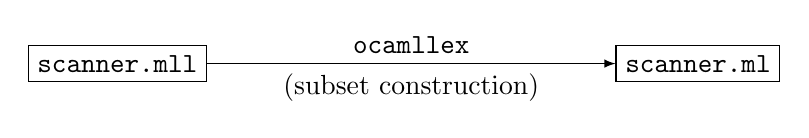
\begin{tikzpicture}
  \node [draw] (mll) {\texttt{scanner.mll}};
  \node [draw,right=15pc] (ml) {\texttt{scanner.ml}};
  \draw [->] (mll) -- node [above] {\texttt{ocamllex}}
                      node [below] {(subset construction)} (ml);
\end{tikzpicture}

An example:

\medskip

scanner.mll

\vspace{4pt}

\begin{ocamllex}
{ open Parser }

rule token =
  parse [' ' '\t' '\r' '\n'] { token lexbuf }
      | '+'                  { PLUS }
      | '-'                  { MINUS }
      | '*'                  { TIMES }
      | '/'                  { DIVIDE }
      | ['0'-'9']+ as lit    { LITERAL(int_of_string lit) }
      | eof                  { EOF }
\end{ocamllex}

\end{frame}

\begin{frame}[fragile]{Ocamllex Specifications}

\begin{ocamllex}
{
  (* Header: verbatim OCaml code; mandatory *)
}

(* Definitions: optional *)
let ident = regexp
let ...

(* Rules: mandatory *)
rule entrypoint1 [arg1 ... argn] =
  parse pattern1 { action (* OCaml code *) }
      | ...
      | patternn { action }
and entrypoint2 [arg1 ... argn]} =
  ...
and ...

{
  (* Trailer: verbatim OCaml code; optional *)
}
\end{ocamllex}

\end{frame}

\begin{frame}[fragile]{Patterns (In Order of Decreasing Precedence)}
\footnotesize
\begin{tabular}{ll}
\toprule
\textbf{Pattern} & \textbf{Meaning} \\
\midrule
\verb|'c'| & A single character\\
\verb|_| & Any character (underline)\\
\verb|eof| & The end-of-file\\
\verb|"foo"| & A literal string\\
\verb|['1' '5' 'a'-'z']| & ``1,'' ``5,'' or any lowercase letter\\
\verb|[^ '0'-'9']| & Any character except a digit \\
\verb|(| \emph{pattern} \verb|)| & Grouping\\
\emph{identifier} & A pattern defined in the \texttt{let} section\\
\midrule
\emph{pattern} \verb|*| & Zero or more \emph{pattern}s\\
\emph{pattern} \verb|+| & One or more \emph{pattern}s\\
\midrule
\emph{pattern} \verb|?| & Zero or one \emph{pattern}s\\
\midrule
\emph{pattern}$_1$ \emph{pattern}$_2$  & \emph{pattern}$_1$ followed by \emph{pattern}$_2$\\
\midrule
\emph{pattern}$_1$ \verb+|+ \emph{pattern}$_2$  & Either \emph{pattern}$_1$ or \emph{pattern}$_2$\\
\midrule
\emph{pattern} \verb|as| \emph{id}  & Bind the matched pattern to variable \emph{id}\\
\bottomrule
\end{tabular}

\end{frame}

\begin{frame}[fragile]{An Example}
\small
\begin{ocamllex}
{ type token = PLUS | IF | ID of string | NUM of int }
let letter = ['a'-'z' 'A'-'Z']
let digit = ['0'-'9']

rule token =
 parse [' ' '\n' '\t'] { token lexbuf } (* Ignore whitespace *)

     | '+' { PLUS }                     (* A symbol *)

     | "if" { IF }                      (* A keyword *)
                                        (* Identifiers *)
     | letter (letter | digit | '_')* as id { ID(id) }
                                        (* Numeric literals *)
     | digit+ as lit { NUM(int_of_string lit) }

     | "/*" { comment lexbuf }          (* C-style comments *)

and comment =
  parse "*/" { token lexbuf } (* Return to normal scanning *)
      | _ { comment lexbuf }  (* Ignore other characters *)
\end{ocamllex}

\end{frame}


\begin{frame}[fragile]{Nested Comments}
\small
\begin{ocamllex}
{ type token = PLUS | ID of string | NUM of int }

let letter = ['a'-'z' 'A'-'Z']
let digit = ['0'-'9']

rule token =
 parse [' ' '\n' '\t'] { token lexbuf } (* Ignore whitespace *)

     | '+' { PLUS }                     (* A symbol *)

     | letter (letter | digit | '_')* as id { ID(id) }
     | digit+ as lit { NUM(int_of_string lit) }

     | "/*" { comment 0 lexbuf }          (* C-style comments *)

and comment level =
  parse "*/" { if level == 0 then token lexbuf
  	else comments (level - 1) lexbuf } 
      | "/*" { comment (level + 1) lexbuf }
      | _ { comment level lexbuf }  (* Ignore other characters *)
\end{ocamllex}

\end{frame}

\begin{frame}{Free-Format Languages}
Typical style arising from scanner/parser division

Program text is a series of tokens possibly separated by whitespace
and comments, which are both ignored.

\begin{itemize}
\item keywords (\texttt{if while})
\item punctuation (\texttt{, ( +})
\item identifiers (\texttt{foo bar})
\item numbers (\texttt{10 -3.14159e+32})
\item strings (\texttt{"A String"})
\end{itemize}

\end{frame}

\begin{frame}{Free-Format Languages}

Java \hfil C \hfil C++ \hfil C\# \hfil Algol \hfil Pascal

Some deviate a little (e.g., C and C++ have a separate preprocessor)

But not all languages are free-format.
\end{frame}

%\begin{frame}[fragile]{FORTRAN 77}
%
%FORTRAN 77 is not free-format.  72-character lines:
%
%\begin{fortran}
%100   IF(IN .EQ. 'Y' .OR. IN .EQ. 'y' .OR.
%     $   IN .EQ. 'T' .OR. IN .EQ. 't') THEN
%\end{fortran}
%
%% $
%
%{
%\[\underbrace{\framebox{\textrm{1}} \cdots \framebox{\textrm{5}}}_{\mbox{Statement label}}
%\underbrace{\framebox{\textrm{6}}}_{\mbox{Continuation}}
%\underbrace{\framebox{\textrm{7}} \cdots \framebox{\textrm{72}}}_{\mbox{Normal}}\]
%}
%
%When column 6 is not a space, line is considered part of the
%previous.
%
%Fixed-length line works well with a one-line buffer.
%
%Makes sense on punch cards. \includegraphics[width=8pc]{punchcard.jpg}
%
%\end{frame}

\begin{frame}[fragile]{Python}

The Python scripting language groups with indentation

\begin{python}
i = 0
while i < 10:
    i = i + 1
    print i    # Prints 1, 2, ..., 10

i = 0
while i < 10:
    i = i + 1
print i        # Just prints 10
\end{python}

This is succinct, but can be error-prone.

How do you wrap a conditional around instructions?

\end{frame}

\begin{frame}[fragile]{Syntax and Language Design}

Does syntax matter?  Yes and no

More important is a language's \emph{semantics}---its meaning.

The syntax is aesthetic, but can be a religious issue.

But aesthetics matter to people, and can be critical.

Verbosity does matter: smaller is usually better.

Too small can be problematic: APL is a succinct language with its
own character set.

There are no APL programs, only puzzles.

\end{frame}

\begin{frame}[fragile]{Syntax and Language Design}

Some syntax is error-prone.  Classic \textsc{fortran} example:

\begin{fortran}
DO 5 I = 1,25  ! Loop header (for i = 1 to 25)
DO 5 I = 1.25  ! Assignment to variable DO5I
\end{fortran}

Trying too hard to reuse existing syntax in C++:

\begin{cpp}
vector< vector<int> > foo;
vector<vector<int>> foo; // Syntax error
\end{cpp}

C distinguishes \verb|>| and \verb|>>| as different operators.

Bjarne Stroustrup tells me they have finally fixed this.

\end{frame}

\end{document}

% Local Variables:
% compile-command: "make syntax.pdf"
% End:
